% =====================================================================
\subsection{Solution}
% =====================================================================

The model is written in Julia with JuMP and solved with Gurobi. It has 50 variables and 35 constraints (not counting the simple bounds).
The solver finds an optimal solution.

\paragraph{Gross margin.}
The optimal gross margin is \textbf{122,077.77 EUR}.

\begin{center}
\small
\begin{tabular}{@{}lr@{}}
\toprule
 & EUR \\
\midrule
Revenue & 248,525.10 \\
Variable crop costs & $-$122,547.32 \\
Pumping cost & $-$900.00 \\
Hired labour & $-$3,000.00 \\
\midrule
Gross margin & 122,077.77 \\
\bottomrule
\end{tabular}
\end{center}

\paragraph{Cropping plan block by block.}
Areas are in hectares. Each row adds up to the area of the block.

\begin{center}
\small
\begin{tabular}{@{}lrrrrrrrr@{}}
\toprule
Block & Wheat & Barley & Maize & Sugar beet & Potato & Beans & Fallow & Total \\
\midrule
B1 (deep loam)  & --- & --- & --- & 11.11 & 14.89 & --- & ---  & 26.00 \\
B2 (silt loam)  & 18.00 & 0.85 & --- & 3.15 & --- & --- & ---  & 22.00 \\
B3 (sandy loam) & --- & 11.30 & 3.50 & --- & --- & --- & 3.20 & 18.00 \\
B4 (heavy clay) & 14.00 & --- & --- & --- & --- & --- & ---  & 14.00 \\
\midrule
Farm & 32.00 & 12.15 & 3.50 & 14.26 & 14.89 & 0.00 & 3.20 & 80.00 \\
Share of farm & 40.0\% & 15.2\% & 4.4\% & 17.8\% & 18.6\% & 0\% & 4.0\% & 100\% \\
\bottomrule
\end{tabular}
\end{center}

Winter wheat is grown on exactly 40\% of the farm, its largest allowed share. Potatoes are grown on the deep loam block B1, where their yield is highest, and not on heavy clay, where it is very low. Field beans are not grown.

\paragraph{Production and sales.}
Everything that is grown is sold. Only the sugar beet and potato contracts have limits.

\begin{center}
\small
\begin{tabular}{@{}lrrr@{}}
\toprule
Crop & Tonnes & Price (EUR/t) & Revenue (EUR) \\
\midrule
Winter wheat  & 302.40  & 210 & 63,504.00 \\
Winter barley & 98.72   & 195 & 19,249.47 \\
Grain maize   & 42.04   & 195 & 8,198.24 \\
Sugar beet    & 1,199.30 & 38  & 45,573.39 \\
Potato        & 700.00  & 160 & 112,000.00 \\
\bottomrule
\end{tabular}
\end{center}

The potato contract ceiling (700 t) is reached exactly. The sugar beet delivery (1,199 t) is above the minimum of 900 t and below the ceiling of 1,700 t, so no spot sales occur.

\paragraph{Use of the reservoir.}

\begin{center}
\small
\begin{tabular}{@{}lrrrrrr@{}}
\toprule
Period & Inflow & Pumped & Pump limit & Irrigation & Lost & Level at end \\
\midrule
Start &      &       &       &        &       & 9,000 \\
P1 spring       & 5,500 & 0     & 5,000 & 0      & 1,500 & 13,000 \\
P2 early summer & 2,000 & 4,000 & 5,000 & 13,786 & 0     & 5,214 \\
P3 late summer  & 1,200 & 5,000 & 5,000 & 11,414 & 0     & 0 \\
P4 autumn       & 9,000 & 1,000 & 5,000 & 0      & 0     & 10,000 \\
\bottomrule
\end{tabular}
\end{center}
All values are in m$^3$.

\begin{itemize}
  \item In spring the reservoir is already almost full (9,000 + 5,500 > 13,000), and no crop needs irrigation, so 1,500 m$^3$ of free water is lost. Nothing is pumped in spring.
  \item In the two summer periods irrigation uses 25,200 m$^3$ in total. It comes from the stock stored in spring, from the inflow, and from 9,000 m$^3$ pumped. The reservoir is \emph{empty} at the end of P3.
  \item In autumn the inflow (9,000 m$^3$) refills the empty reservoir, and 1,000 m$^3$ more are pumped to reach the required end level of 10,000 m$^3$.
  \item The whole permit of 10,000 m$^3$ is used (pumping cost 900 EUR).
\end{itemize}

\paragraph{Use of hired labour.}

\begin{center}
\small
\begin{tabular}{@{}lrrrrr@{}}
\toprule
Period & Hours needed & Family hours & Hired & Hiring limit & Wage bill (EUR) \\
\midrule
P1 spring       & 328.3 & 520 & 0   & 200 & 0 \\
P2 early summer & 204.4 & 470 & 0   & 200 & 0 \\
P3 late summer  & 281.2 & 500 & 0   & 250 & 0 \\
P4 autumn       & 545.0 & 420 & 125 & 125 & 3,000 \\
\bottomrule
\end{tabular}
\end{center}

The family is enough in the first three periods. Hired labour is used only in autumn, when the potato harvest needs 18 hours per hectare. All 125 hired hours are used (the hiring limit), and they cost 24 EUR per hour.

\begin{figure}[h]
\centering
\begin{minipage}{0.48\textwidth}
\centering
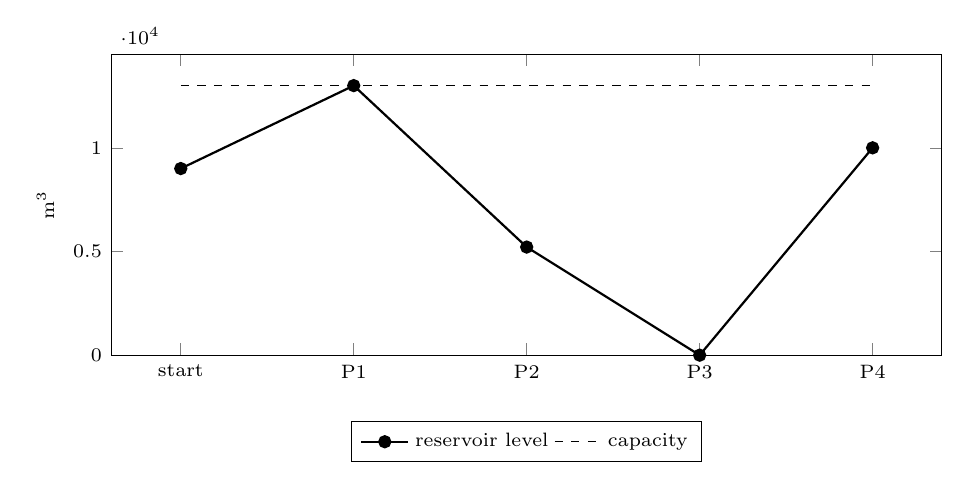
\begin{tikzpicture}
\begin{axis}[
  width=\linewidth, height=5.4cm,
  symbolic x coords={start,P1,P2,P3,P4}, xtick=data,
  ymin=0, ymax=14500, ylabel={m$^3$},
  legend style={font=\scriptsize, at={(0.5,-0.22)}, anchor=north, legend columns=-1},
  tick label style={font=\scriptsize}, label style={font=\scriptsize}]
\addplot[thick, mark=*] coordinates {(start,9000) (P1,13000) (P2,5214) (P3,0) (P4,10000)};
\addplot[dashed] coordinates {(start,13000) (P4,13000)};
\legend{reservoir level, capacity}
\end{axis}
\end{tikzpicture}

\small (a) Reservoir level at the end of each period
\end{minipage}\hfill
\begin{minipage}{0.48\textwidth}
\centering
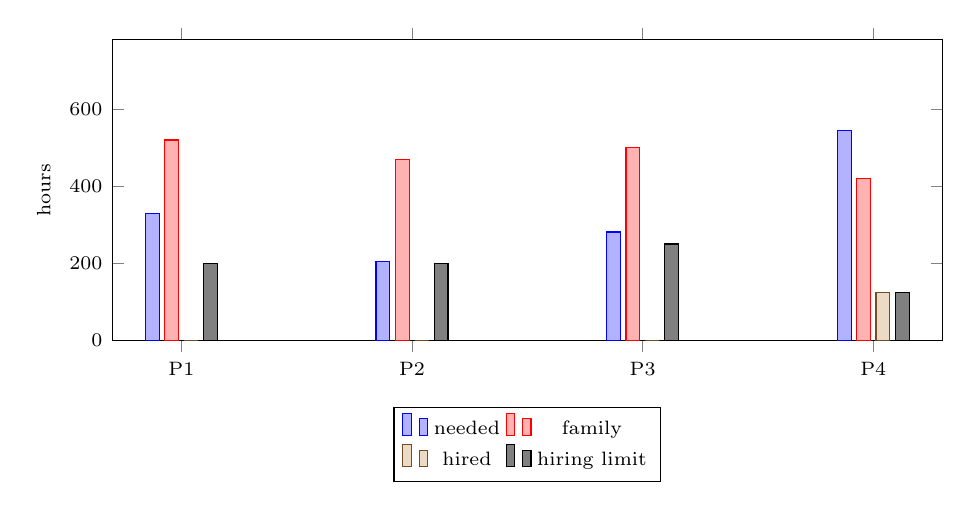
\begin{tikzpicture}
\begin{axis}[
  width=\linewidth, height=5.4cm,
  ybar, bar width=5pt,
  symbolic x coords={P1,P2,P3,P4}, xtick=data,
  ymin=0, ymax=780, ylabel={hours},
  legend style={font=\scriptsize, at={(0.5,-0.22)}, anchor=north, legend columns=2},
  tick label style={font=\scriptsize}, label style={font=\scriptsize}]
\addplot coordinates {(P1,328.3) (P2,204.4) (P3,281.2) (P4,545.0)};
\addplot coordinates {(P1,520) (P2,470) (P3,500) (P4,420)};
\addplot coordinates {(P1,0) (P2,0) (P3,0) (P4,125)};
\addplot coordinates {(P1,200) (P2,200) (P3,250) (P4,125)};
\legend{needed, family, hired, hiring limit}
\end{axis}
\end{tikzpicture}

\small (b) Work needed, family hours and hired hours
\end{minipage}
\caption{How the optimal plan uses the reservoir and the hired labour.}
\label{fig:water-labour}
\end{figure}


\paragraph{Which resources are exhausted?}

\begin{center}
\small
\begin{tabular}{@{}p{0.47\textwidth}p{0.47\textwidth}@{}}
\toprule
\textbf{Exhausted (at the limit)} & \textbf{Not exhausted (slack left)} \\
\midrule
Land: all 80 ha are sown &
Pump in P1 (0 of 5,000), P2 (4,000 of 5,000) and P4 (1,000 of 5,000) \\
Abstraction permit: 10,000 of 10,000 m$^3$ &
Family hours in P1, P2, P3 (slack 192, 266 and 219 h) \\
Pump in P3: 5,000 of 5,000 m$^3$ &
Hired hours in P1, P2, P3 (none needed) \\
Reservoir full at the end of P1 (13,000 m$^3$) &
Share limit of barley, maize, sugar beet, potato (slack 19.9, 28.5, 17.7 and 17.1 ha) \\
Reservoir empty at the end of P3 &
Sugar beet: contract ceiling (1,199 of 1,700 t) and minimum (1,199 of 900 t) \\
Reservoir end level: exactly 10,000 m$^3$ &
Reservoir capacity in P2 and P4 \\
Family hours in P4: 420 of 420 h & \\
Hired hours in P4: 125 of 125 h & \\
Share limit of winter wheat: 32 of 32 ha & \\
Potato contract ceiling: 700 of 700 t & \\
Non-productive area: 3.2 of 3.2 ha & \\
\bottomrule
\end{tabular}
\end{center}

In short, water is the main shortage (permit, summer pump and empty reservoir), and autumn labour is the second one. The plan also meets the wheat share limit and the potato contract ceiling.
